%(BEGIN_QUESTION)
% Copyright 2008, Tony R. Kuphaldt, released under the Creative Commons Attribution License (v 1.0)
% This means you may do almost anything with this work of mine, so long as you give me proper credit

En presisjonsvekt med balansearm brukes på et legekontor for å veie pasienter. Lodd plasseres på enden av armen til balansen igjen er i likevekt. Antall lodd på armen blir da en representasjon av pasientens vekt:

$$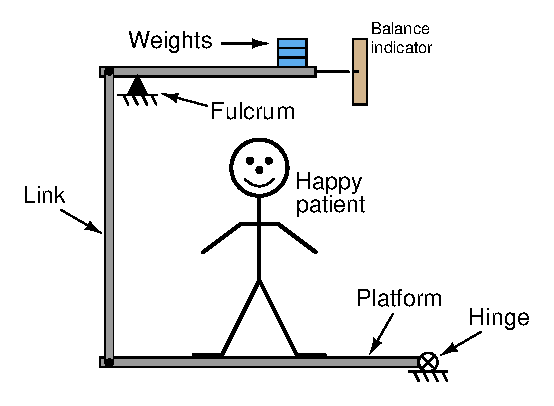
\includegraphics[width=15.5cm]{i00466x01.eps}$$

Legen er imidlertid lat. Han vil ikke lenger legge på loddene manuelt for hver pasient. I stedet ønsker han et instrument på kontoret sitt som viser pasientvekten direkte, slik at han slipper å forlate stolen.

\vskip 10pt

\noindent
Det gis poeng for å bestemme følgende:

\begin{itemize}
\item{} Identifiser om den grunnleggende vektmekanismen bygger på {\it kraftbalanse}-prinsippet eller {\it bevegelsesbalanse}-prinsippet
\item{} Skisser riktig plassering av en flapper/nozzle-enhet
\item{} Skisser riktig plassering av en tilbakekoblingsbelg
\item{} Skisser riktige pneumatiske rørforbindelser mellom en restriktor, dysen, belgen og instrumentet på legekontoret
\end{itemize}

Du kan gjerne tegne svaret direkte på dette diagrammet (uten lodd og indikator):

\vskip 40pt

$$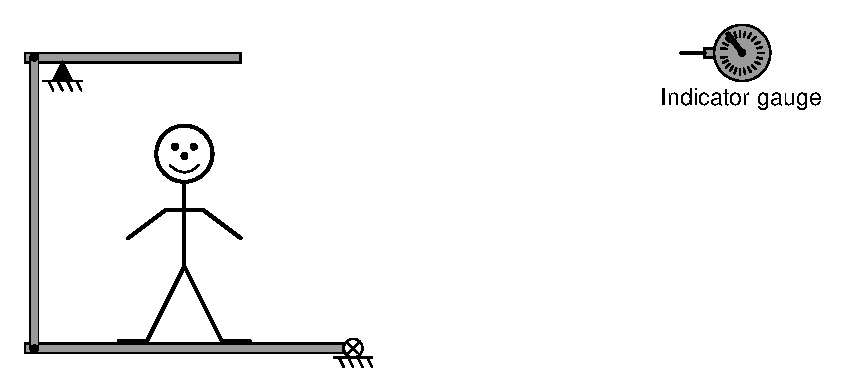
\includegraphics[width=15.5cm]{i00466x02.eps}$$

\underbar{file i00466}
%(END_QUESTION)





%(BEGIN_ANSWER)

(2 poeng): Vekten fungerer etter {\bf kraftbalanse}-prinsippet

\vskip 10pt

Dette er bare én mulig løsning -- det finnes flere!

$$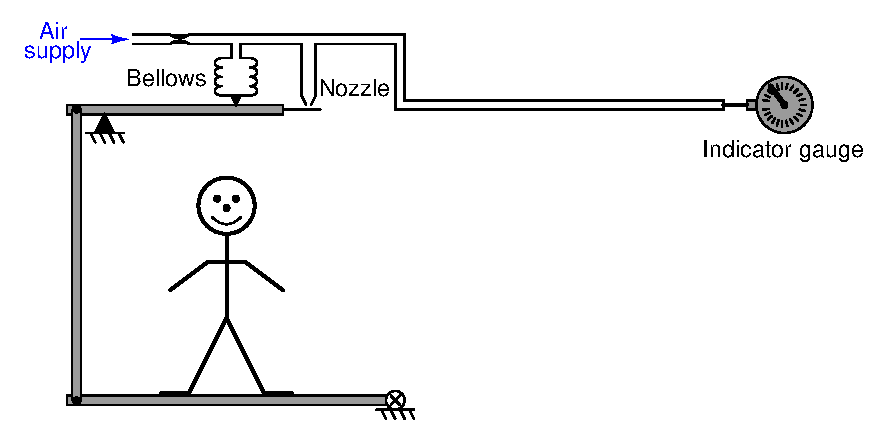
\includegraphics[width=15.5cm]{i00466x03.eps}$$

Gi 2 poeng for fungerende plassering av flapper/nozzle, 2 poeng for fungerende tilbakekoblingsbelg, og 4 poeng for resten (rør, restriktor, instrument, forsyning)

%(END_ANSWER)





%(BEGIN_NOTES)

{\bf Denne oppgaven er ment for eksamen, ikke arbeidsark!}.

%(END_NOTES)
